% AER: Insights submission: anonymised manuscript.
% Sections in aeri/sections/: edit them directly. They are a separate copy, so changes to the working paper (sections/) do not carry over.
% aeri_wordcount.tex compiles this file without title, abstract, exhibits and references (for the AEA word-count tool).
\documentclass[11pt]{article}

\usepackage[margin=1in]{geometry}
\usepackage[T1]{fontenc}
\usepackage[utf8]{inputenc}
\usepackage{lmodern}
\usepackage{microtype}
\usepackage{amsmath}
\usepackage{amssymb}
\usepackage{booktabs}
\usepackage{array}
\usepackage{threeparttable}
\usepackage{graphicx}
\usepackage{xcolor}
\usepackage{caption}
\usepackage{etoolbox}
\usepackage[section]{placeins}                        % floats stay in their own section
\renewcommand{\topfraction}{0.9}\renewcommand{\textfraction}{0.07}\renewcommand{\floatpagefraction}{0.75}
\usepackage[authoryear,round]{natbib}
\usepackage[hidelinks]{hyperref}
\usepackage{setspace}
\onehalfspacing

\captionsetup{font=small, labelfont=bf, skip=4pt}
\newcommand{\SuppTab}[2]{Supplemental Appendix Table~#1}
\newcommand{\figurenotes}[1]{\par\vspace{2pt}{\footnotesize\leftskip=0pt\rightskip=0pt\parfillskip=0pt plus 1fil\noindent\emph{Notes:} #1\par}}

\ifdefined\aeriwordcount
  \makeatletter                                       % exhibits typeset into a discarded box: not counted
  \AtBeginDocument{%
    \renewenvironment{table}[1][]{\def\@captype{table}\setbox0=\vbox\bgroup}{\egroup}%
    \renewenvironment{figure}[1][]{\def\@captype{figure}\setbox0=\vbox\bgroup}{\egroup}}
  \makeatother
  \usepackage{bibentry}                             % citations resolve, reference list not printed
\else
  \AtBeginEnvironment{table}{\singlespacing}\AtBeginEnvironment{figure}{\singlespacing}
\fi

\begin{document}

\ifdefined\aeriwordcount\else
\begin{center}
{\Large\textbf{The Invention or the Inventor?\\Owner Constraints and Patent Value in Emerging Markets}}
\end{center}

\begin{abstract}
\noindent Are emerging-market patents worth less because the inventions are weaker or because their owners cannot
use them? Using renewal records for 2.6 million firm and university patents from 2000--2005 in five emerging and five advanced
economies, I compare domestic and foreign owners within each office. At equal citations, field and grant lag,
emerging-market firms keep their patents as long as comparable rich-economy firms, and credit crunches do not
raise their lapses. Chinese universities are the exception. Patents that small Chinese firms and universities sell to
unrelated buyers survive far longer: markets for technology, not fee relief, matter.

\medskip
\noindent\textbf{JEL codes:} O34, O31, O32, O57, L26\\
\noindent\textbf{Keywords:} patent renewal; patent value; emerging markets; markets for technology
\end{abstract}
\fi

\section{Introduction}

Emerging economies now account for a large share of the world's patenting: China's patent office alone received
49\% of the 3.7 million patent applications filed worldwide in 2024, up from 35\% in 2014 \citep{WIPO2025}. Yet
their patents are widely thought to be worth less. Renewal decisions offer a direct test. Owners pay a fee every year to keep a patent in force and stop paying
once it is no longer worth the fee, so the age at which patents lapse reveals what they are worth to their owners
\citep{PakesSchankerman1984,Pakes1986,SchankermanPakes1986}. By this measure the gap looks large. Among patents
filed in 2000--2005, domestic owners' patents fall short of foreign owners' patents in survival eight years after
grant by 12 percentage points more in the emerging-market offices than in the advanced ones.

Two very different stories fit such a gap. In the first, the \emph{invention} is the problem: emerging-market
patents protect weaker technology, and owners rationally drop them sooner. In the second, the \emph{inventor} is
the problem: owners lack the finance, production capacity or market access to turn valuable inventions into
returns, so good patents lapse for want of an owner able to use them. The policy responses differ. The first calls
for investment in research capability and links to frontier technology; the second for credit, fee relief or
markets in which patents can find better owners.

This paper separates the two using the legal-event records in PATSTAT,\footnote{PATSTAT is the European Patent Office's worldwide patent statistical database.} which track renewals and lapses at the
offices that report them. I first establish which offices do: of the large emerging economies, only China, Korea,
Russia, Brazil and the Czech Republic record lapses consistently and have enough domestic firm
patents.\footnote{Most countries in Latin America, Africa and South-East Asia report no lapses
to PATSTAT; Hungary reports them but has too few domestic firm patents, and Taiwan was already a high-income economy (Supplemental Appendix~S1).}
I compare these against five advanced economies (the United States, Japan, Germany, the United Kingdom, and France) using 2.5 million granted patents held by firms and universities, and renewal-fee schedules from official sources. The design compares domestic and foreign owners in the same office (exposed to the same fees, law and
enforcement), and asks whether the domestic shortfall is larger in emerging-market offices. The paper makes four
points.

First, the raw shortfall reflects what is patented. Domestic patents in emerging-market offices are cited far less
than foreign ones and are granted sooner. Comparing patents with the same citations, technology field and grant lag,
emerging-market firms keep their patents about as long as comparable firms in the advanced economies
(Section~\ref{sec:survival}): small firms are level, and mid-sized and large firms 5--8 percentage points ahead.
Office by office, Chinese small firms are level, Korean firms ahead and Russian firms
behind.

Second, three tests look for owner constraints (Section~\ref{sec:constraints}). Two find none: owners keep the home
patent of an invention longer than its foreign patents, more so in the emerging economies, and credit crunches do not
raise emerging-market firms' lapses. The third points to owner capacity at the margin: patents that small Chinese
firms sell to unrelated buyers survive 11 points longer afterwards, against little in Germany and France, although the
comparison rests on few sales there. Small Chinese firms also barely respond to fee cuts.

Third, renewal models turn these decisions into money (Section~\ref{sec:values}). Valuing each patent from its own
renewal history, without reference to its owner, the home premium (the value of domestic relative to foreign owners'
patents in the same office) does not differ significantly between the emerging-market and the advanced offices for
all owners and for large firms, and is larger in the emerging-market offices for mid-sized firms. For small firms it
is smaller against the advanced-economy pool, which Japan dominates; office by office, it is 29\% in China and 65\%
in Korea, against 28\% in the United States and 31\% in Germany.

Fourth, Chinese universities are the clear weak spot. Their patents are 15 points less likely than foreign
universities' patents in China to be alive eight years after grant and are worth 59\% less at equal citations. Here
the owner matters: once sold to an unrelated firm, Chinese university patents survive 45 points longer.

I close by pricing the policy levers on a common scale (Section~\ref{sec:stake}). Had every eligible owner taken up
China's, Korea's and Brazil's fee discounts, the returns from a cohort of patents would have risen by about a million
dollars or less. Had small Chinese firms' patents earned what they earn in buyers' hands, returns would have risen by up to
\$130 million per cohort, or \$280 million with mid-sized firms; moving Chinese university patents to firms is worth
up to \$460 million, and raising their returns to what foreign universities' patents earn in China at equal
citations, \$180--320 million. These are
rough private returns, not welfare, but the ordering is clear: the gains lie in markets for technology and in what
universities patent, not in cheaper renewal.

The paper contributes to three literatures. The first estimates the value of patent rights from renewal decisions
\citep{PakesSchankerman1984,Pakes1986,SchankermanPakes1986,Lanjouw1998,Schankerman1998,LanjouwPakesPutnam1998,Bessen2008}
and the role of fees \citep{deRassenfosseVanPottelsberghe2013}; I extend it to emerging-market
offices, with fee histories for ten offices over 25 years. The second studies indicators of patent value
\citep{HarhoffSchererVopel2003,HallJaffeTrajtenberg2005,KoganEtAl2017}; I value each patent from its own renewal
path rather than from its owner's characteristics. The third asks whether Chinese and other emerging-market patenting
is of low quality \citep{HuJefferson2009,LiegsalzWagner2013,DangMotohashi2015,HuZhangZhao2017,WeiXieZhang2017}; the answer here is that, for firms,
lower survival on average reflects the technology rather than the owners' ability to use their patents, although
owner capacity matters at the margin. The sale premium connects to
work on markets for technology
\citep{AroraFosfuriGambardella2001,Serrano2010,Serrano2018,GalassoSchankermanSerrano2013,AkcigitCelikGreenwood2016},
and the university result to work on who should own university inventions \citep{HvideJones2018}.

\section{Data and design}\label{sec:data}

\paragraph{Patents and lapses.} The data are PATSTAT Global \citep[autumn 2025 edition;][]{PATSTAT}. The sample is
granted invention patents filed in 2000--2005 at ten national offices, followed for up to twenty years (to 2019 in Korea and 2022 in Russia, where the
lapse records end). A patent
lapses if the INPADOC legal-event table records its first cessation within 19.5 years of filing; a later cessation
marks expiry at full term. I chose the offices by scanning every authority in the legal-event table for the share of
grants with a recorded cessation and the continuity of records over time (Supplemental Appendix~S1). The
emerging-market offices are those of China, Korea, Russia, Taiwan and the Czech Republic; the advanced-economy
offices are those of the United States, Japan, Germany, the United Kingdom and France. Between them, the five
emerging-market offices granted 84\% of the invention patents filed in 2000--2005 at the national offices of
emerging economies in PATSTAT, and the five advanced-economy offices 88\% of those filed at the national offices of
advanced economies.\footnote{Advanced economies as listed by the IMF in 2005, without Korea and Taiwan; regional offices
such as the European Patent Office are left out.}

\paragraph{Owners.} An owner is domestic if the first applicant is from the office's country. Missing applicant
countries (common in China and Japan) are imputed from the patent family and the office of first filing. Owners are
grouped by sector and size. Size is the number of distinct inventions (DOCDB families) the harmonised applicant filed
worldwide in 2000--2005, the cohort's own filing window, so that it is measured before the outcomes: small firms have
1--9 inventions, mid-sized firms 10--99 and large firms 100 or more; universities and public research organisations
form a fourth group. Individual inventors are excluded: their patents behave differently, and in China they were the
main target of local filing subsidies in this period. Patents granted more than ten years after filing are dropped.
Table~\ref{tab:sample} describes the sample: patents by office and owner in panel A, owners in panel B. It
covers 194{,}518 small firms, 28{,}657 mid-sized firms, 4{,}487 large firms and 17{,}151 universities and public
research organisations, each owner counted once whether it is domestic or foreign.

\begin{table}[t]
\centering
\begin{threeparttable}
\caption{The sample: granted patents filed 2000--2005, firms and universities}\label{tab:sample}
\small
% Source: em-patent-value output/sample_counts.csv (29_sample_tables.py)
\setlength{\tabcolsep}{4pt}
\begin{tabular}{lrrrrrrrrr}
\toprule
 & & \multicolumn{4}{c}{Domestic owners} & \multicolumn{4}{c}{Foreign owners} \\
\cmidrule(lr){3-6}\cmidrule(lr){7-10}
 & & \multicolumn{3}{c}{Firms} & & \multicolumn{3}{c}{Firms} & \\
\cmidrule(lr){3-5}\cmidrule(lr){7-9}
Office & Patents & Small & Mid & Large & Univ. & Small & Mid & Large & Univ. \\
\midrule
\multicolumn{10}{l}{\emph{A. Patents, by office}} \\
China          &   363{,}574 & 26{,}155 & 12{,}411 &  27{,}983 & 39{,}836 & 41{,}845 & 40{,}870 & 143{,}289 &  3{,}982 \\
Korea          &   371{,}332 & 33{,}505 & 21{,}556 & 157{,}473 & 19{,}530 &  8{,}283 & 16{,}088 &  50{,}457 &  1{,}248 \\
Russia         &   129{,}038 & 10{,}130 &  3{,}397 &       841 & 15{,}738 &  8{,}202 &  6{,}144 &   4{,}993 &      467 \\
Taiwan         &   150{,}743 &  6{,}038 &  8{,}190 &  28{,}420 &  6{,}665 &  7{,}510 & 15{,}834 &  76{,}313 &      916 \\
Czech Rep.     &     4{,}061 &      584 &      325 &        -- &       95 &      571 &      826 &   1{,}249 &       24 \\
\addlinespace
United States  &   980{,}998 & 77{,}598 & 87{,}443 & 274{,}701 & 28{,}373 & 47{,}953 & 66{,}673 & 338{,}738 & 17{,}002 \\
Japan          &   775{,}826 & 23{,}780 & 55{,}011 & 539{,}643 & 15{,}540 &  5{,}561 &  9{,}718 &  27{,}163 &  1{,}141 \\
Germany        &    81{,}937 & 11{,}218 & 15{,}326 &  33{,}302 &  3{,}587 &  1{,}669 &  3{,}104 &  13{,}403 &      210 \\
United Kingdom &    41{,}383 &  6{,}095 &  4{,}085 &   1{,}730 &      445 &  3{,}219 &  5{,}028 &  19{,}964 &      591 \\
France         &    62{,}937 & 11{,}228 & 10{,}448 &  21{,}569 &  3{,}753 &  1{,}465 &  1{,}957 &   8{,}368 &      162 \\
\midrule
Total          & 2{,}961{,}829 & 206{,}331 & 218{,}192 & 1{,}085{,}662 & 133{,}562 & 126{,}278 & 166{,}242 & 683{,}937 & 25{,}743 \\
\midrule
\multicolumn{10}{l}{\emph{B. Owners, by office}} \\
% Source: em-patent-value output/owner_counts.csv (29b_owner_counts.py)
China          &   & 18{,}838 & 1{,}014 & 157 & 6{,}122 & 30{,}420 & 7{,}518 & 2{,}084 & 1{,}738 \\
Korea          &   & 18{,}996 & 1{,}798 & 243 & 732 & 5{,}607 & 3{,}730 & 1{,}592 & 433 \\
Russia         &   & 6{,}121 & 176 & 5 & 3{,}679 & 4{,}735 & 407 & 93 & 289 \\
Taiwan         &   & 3{,}513 & 563 & 82 & 183 & 5{,}255 & 3{,}295 & 1{,}209 & 270 \\
Czech Rep.     &   & 373 & 19 & -- & 55 & 472 & 465 & 291 & 23 \\
\addlinespace
United States  &   & 42{,}360 & 5{,}853 & 787 & 1{,}369 & 32{,}868 & 8{,}435 & 1{,}448 & 2{,}129 \\
Japan          &   & 15{,}610 & 6{,}588 & 1{,}684 & 497 & 3{,}674 & 1{,}284 & 510 & 282 \\
Germany        &   & 7{,}270 & 1{,}993 & 299 & 341 & 1{,}246 & 830 & 545 & 79 \\
United Kingdom &   & 3{,}916 & 531 & 44 & 145 & 2{,}399 & 1{,}451 & 767 & 210 \\
France         &   & 6{,}292 & 739 & 99 & 296 & 1{,}071 & 634 & 474 & 60 \\
\midrule
All offices    &   & 123{,}285 & 19{,}258 & 3{,}365 & 13{,}410 & 78{,}990 & 16{,}172 & 3{,}015 & 4{,}510 \\
\bottomrule
\end{tabular}
\begin{tablenotes}\footnotesize
\item \emph{Notes:} Granted invention patents filed 2000--2005 with a grant lag of up to ten years; individual
owners excluded. Patents: all firms, universities and owners of unknown type. Firm size: inventions (DOCDB families)
filed worldwide by the harmonised applicant in 2000--2005; small 1--9, mid-sized 10--99, large 100 or more; no Czech
firm reaches 100. Univ.: universities and public research organisations. Panel B: distinct harmonised applicants with at
least one sample patent in the office. An owner patenting in several offices is counted in each; All offices counts
it once among domestic and once among foreign owners, so the domestic and foreign totals overlap and fall short
of the sums over offices (an owner whose patents name applicants from different countries can be domestic in more
than one office). Source: PATSTAT Global, autumn 2025.
\end{tablenotes}
\end{threeparttable}
\end{table}



\paragraph{Quality.} Observable quality is measured by forward citations to the patent family (logged) and the
WIPO technology field (35 fields), the controls in the main estimates. Robustness checks add citations in search
reports that block later claims (categories X and Y), citations received in the four years after filing, the grant
lag and family size. Domestic patents in emerging-market offices are cited far less than foreign ones,
by a factor of five in China and six in Korea, so quality controls matter.

\paragraph{Design.} The basic comparison is between domestic and foreign owners in the same office, which holds
fees, law and enforcement fixed. Foreign owners are mostly multinationals protecting a foreign market, so domestic
and foreign patents differ everywhere; the question is whether the domestic shortfall is larger in emerging-market
offices. For patent $i$ of owner group $g$ in office $o$, filed in year $t$ in field $f$,
\begin{equation}\label{eq:did}
  y_{i} = \beta\, D_i + \delta\, D_i \times EM_o + \theta_o \ln(1+c_i) + \mu_{ot} + \lambda_{of} + \kappa_{og}
  + \varepsilon_i ,
\end{equation}
where $y_i$ indicates that the patent is alive eight years after grant,\footnote{Survival is measured from
grant because renewal fees are due from grant. Grant lags differ across offices and between domestic and foreign
owners in the same office (Supplemental Appendix Figure~S1), so a fixed age from filing would
compare patents that have faced different numbers of renewal decisions.} $D_i$ marks a domestic owner, $EM_o$ an
emerging-market office and $c_i$ citations. The coefficient of interest, $\delta$, is the extra domestic--foreign gap
in emerging-market offices, in percentage points. Standard errors are clustered by owner.

\section{Survival at equal quality}\label{sec:survival}

\paragraph{Main estimates.} Table~\ref{tab:survival} reports $\delta$ in equation~\eqref{eq:did}, the extra
domestic--foreign gap in emerging-market offices. Across the ten offices and for all firms and universities together,
without quality controls it is $-10.1$ points (column 1). Comparing patents with the same citations, technology field
and owner group, it becomes $+4.1$ (column 2): the raw shortfall reflects that domestic patents in emerging-market
offices are much less cited than foreign ones. Columns 3--6 estimate it separately for each owner group. Measured against foreign owners in the same office,
emerging-market firms of every size keep their patents longer than advanced-economy firms do: small firms by 2.8 points,
mid-sized firms by 7.9 and large firms by 9.0. Universities are behind, at $-5.7$, though not significantly.

\paragraph{Which offices drive it.} China and the United States are the largest offices on each side, so
the lower two blocks of Table~\ref{tab:survival} separate them. China against the
United States alone gives the same pooled estimate, $+3.9$, with Chinese small firms 5.4 points ahead and
Chinese universities 15.3 points behind. Without China and the United States the pooled estimate is close to
zero, $-1.0$; mid-sized and large firms are still ahead, by 2.4 and 3.5 points, the second not
significantly, but small firms in Korea, Russia, Taiwan
and the Czech Republic are 4.4 points behind small firms in Japan, Germany, the United Kingdom and France. The
benchmark matters here: small Japanese firms' patents are 18 points more likely to be alive than foreign owners' patents
in Japan, by far the largest domestic advantage among the advanced-economy offices (Supplemental Appendix Table~S4), and
without the United States Japan sets the bar.

\begin{table}[t]
\centering
\caption{Extra domestic--foreign survival gap in emerging-market offices}\label{tab:survival}
\small
% Generated by em-patent-value code/38_paper_exhibits.py (main_table2.csv, step 37); do not edit by hand
\begin{tabular*}{\linewidth}{@{\extracolsep{\fill}}lcccccc}
\toprule
Alive 8 years after grant & \multicolumn{2}{c}{All owners} & Small & Mid-sized & Large & \\
 & & & firms & firms & firms & Universities \\
\cmidrule(lr){2-3}
 & (1) & (2) & (3) & (4) & (5) & (6) \\
\midrule
\multicolumn{7}{l}{\emph{All ten offices}} \\
Domestic owner $\times$ EM office & $-12.3^{***}$ & $3.5^{*}$ & $0.5$ & $8.0^{***}$ & $5.4^{**}$ & $-14.2^{***}$ \\
 & (1.7) & (1.8) & (0.7) & (1.3) & (2.5) & (2.9) \\
Domestic owner & $3.8^{***}$ & $5.0^{***}$ & $3.8^{***}$ & $5.4^{***}$ & $5.0^{***}$ & $4.9^{**}$ \\
 & (0.9) & (1.0) & (0.3) & (0.4) & (1.3) & (2.2) \\
Observations & 2{,}504{,}283 & 2{,}504{,}279 & 255{,}234 & 288{,}177 & 1{,}808{,}726 & 152{,}115 \\
\addlinespace
\multicolumn{7}{l}{\emph{Excl. China and US}} \\
Domestic owner $\times$ EM office & $-9.8^{***}$ & $0.9$ & $-4.8^{***}$ & $5.1^{**}$ & $1.7$ & $-14.4^{**}$ \\
 & (2.2) & (2.4) & (1.5) & (2.0) & (3.1) & (6.1) \\
Domestic owner & $4.9^{***}$ & $8.8^{***}$ & $8.0^{***}$ & $8.1^{***}$ & $9.0^{***}$ & $16.8^{***}$ \\
 & (1.2) & (1.2) & (0.8) & (1.0) & (1.6) & (4.7) \\
Observations & 1{,}229{,}431 & 1{,}229{,}427 & 101{,}703 & 126{,}004 & 938{,}771 & 62{,}922 \\
\addlinespace
\multicolumn{7}{l}{\emph{China and US only}} \\
Domestic owner $\times$ EM office & $-15.3^{***}$ & $3.6$ & $2.6^{***}$ & $10.3^{***}$ & $6.8$ & $-19.7^{***}$ \\
 & (2.6) & (2.8) & (0.8) & (1.7) & (4.4) & (2.8) \\
Domestic owner & $3.4^{***}$ & $3.8^{***}$ & $2.3^{***}$ & $3.6^{***}$ & $3.4^{*}$ & $4.7^{**}$ \\
 & (1.0) & (1.4) & (0.4) & (0.5) & (1.9) & (2.1) \\
Observations & 1{,}274{,}852 & 1{,}274{,}852 & 153{,}531 & 162{,}173 & 869{,}955 & 89{,}193 \\
\midrule
\multicolumn{7}{l}{\emph{Controls (by office)}} \\
\quad Filing year & \checkmark & \checkmark & \checkmark & \checkmark & \checkmark & \checkmark \\
\quad Field, citation bin, grant lag & & \checkmark & \checkmark & \checkmark & \checkmark & \checkmark \\
\quad Domestic $\times$ grant lag & & \checkmark & \checkmark & \checkmark & \checkmark & \checkmark \\
\quad Owner group & & \checkmark & -- & -- & -- & -- \\
\bottomrule
\end{tabular*}

\vspace{4pt}
\begin{minipage}{\linewidth}\footnotesize\emph{Notes:} Linear probability models of survival eight years after grant; granted patents of firms and universities filed 2000--2005, grant lag up to ten years; coefficients in percentage points. The coefficient on domestic owner $\times$ EM office is $\delta$ in equation~\eqref{eq:did}: the extra domestic--foreign gap in the emerging-market offices (China, Korea, Russia, Taiwan, Czech Republic) relative to the advanced-economy offices (United States, Japan, Germany, United Kingdom, France). Column 1: office $\times$ filing-year effects only. Columns 2--6: office-specific effects of filing year, technology field (35), citation bin (forward citations to the family: 0, 1, 2, 3--4, 5--9, 10--19, 20 or more) and grant lag in whole years, a common domestic $\times$ grant-lag slope, and in column 2 office $\times$ owner-group effects; columns 3--6 are estimated separately for each owner group. The domestic-owner coefficient is the advanced-economy gap at the mean grant lag. Firm size: inventions filed worldwide in 2000--2005 by the owner. Standard errors clustered by owner in parentheses; inference across offices in \SuppTab{S3}{tab:rich}. $^{*}$~$p<0.1$, $^{**}$~$p<0.05$, $^{***}$~$p<0.01$.
\end{minipage}
\end{table}


\paragraph{Richer quality controls.} Citations are a noisy measure of quality. Adding citations that block later
claims, citations received in the four years after filing and office-specific slopes in the grant lag lowers the estimates for every
firm size by 1--3 points (Supplemental Appendix Table~S3). Small emerging-market firms then come out level ($-0.4$), or 1.7 points behind when family size is also held
fixed, although family size itself partly reflects an owner's capacity to file abroad;
mid-sized and large firms remain 4--8 points ahead.

\clearpage
\newpage 
\paragraph{By country.} Supplemental Appendix Table~S2 compares each emerging-market office with the five advanced-economy
offices, with the specifications of Table~\ref{tab:survival}. Chinese and Korean firms of every size are ahead: small firms by 4.0 and 5.1
points, larger firms by 7--11 points. Small Czech firms are ahead by a similar amount, 6.3 points, though not
significantly. Russia is the exception: small Russian firms are 4.3 points behind, and Russian universities 11.9. Small
Taiwanese firms are 2.4 points behind, while larger Taiwanese firms and universities are ahead. For all owners
together, Korea and Taiwan are ahead, China and the Czech Republic level and Russia behind; in China, domestic firms'
advantage is offset by universities, 16.9 points behind.
Within each office, the domestic--foreign gap for small firms is close to zero in Russia and Taiwan, against about 2--18
points in the advanced-economy offices (Supplemental Appendix Table~S4).

\section{Are emerging-market owners constrained?}\label{sec:constraints}

Equal survival at equal quality does not rule out owner constraints: constrained owners might keep their patents as
long as others but get less from them, or drop patents that would be worth keeping in other hands. Three tests look
for constraints directly (Figure~\ref{fig:constraints}). Each is shown for all firms, small firms and universities, for the emerging and the
advanced economies separately, and as the difference between the two, which is the test of interest. Country-level
results are in Supplemental Appendix Figure~S2, and a fourth test based on fee changes in Supplemental Appendix
Table~S6.

\begin{figure}[!htbp]
\centering
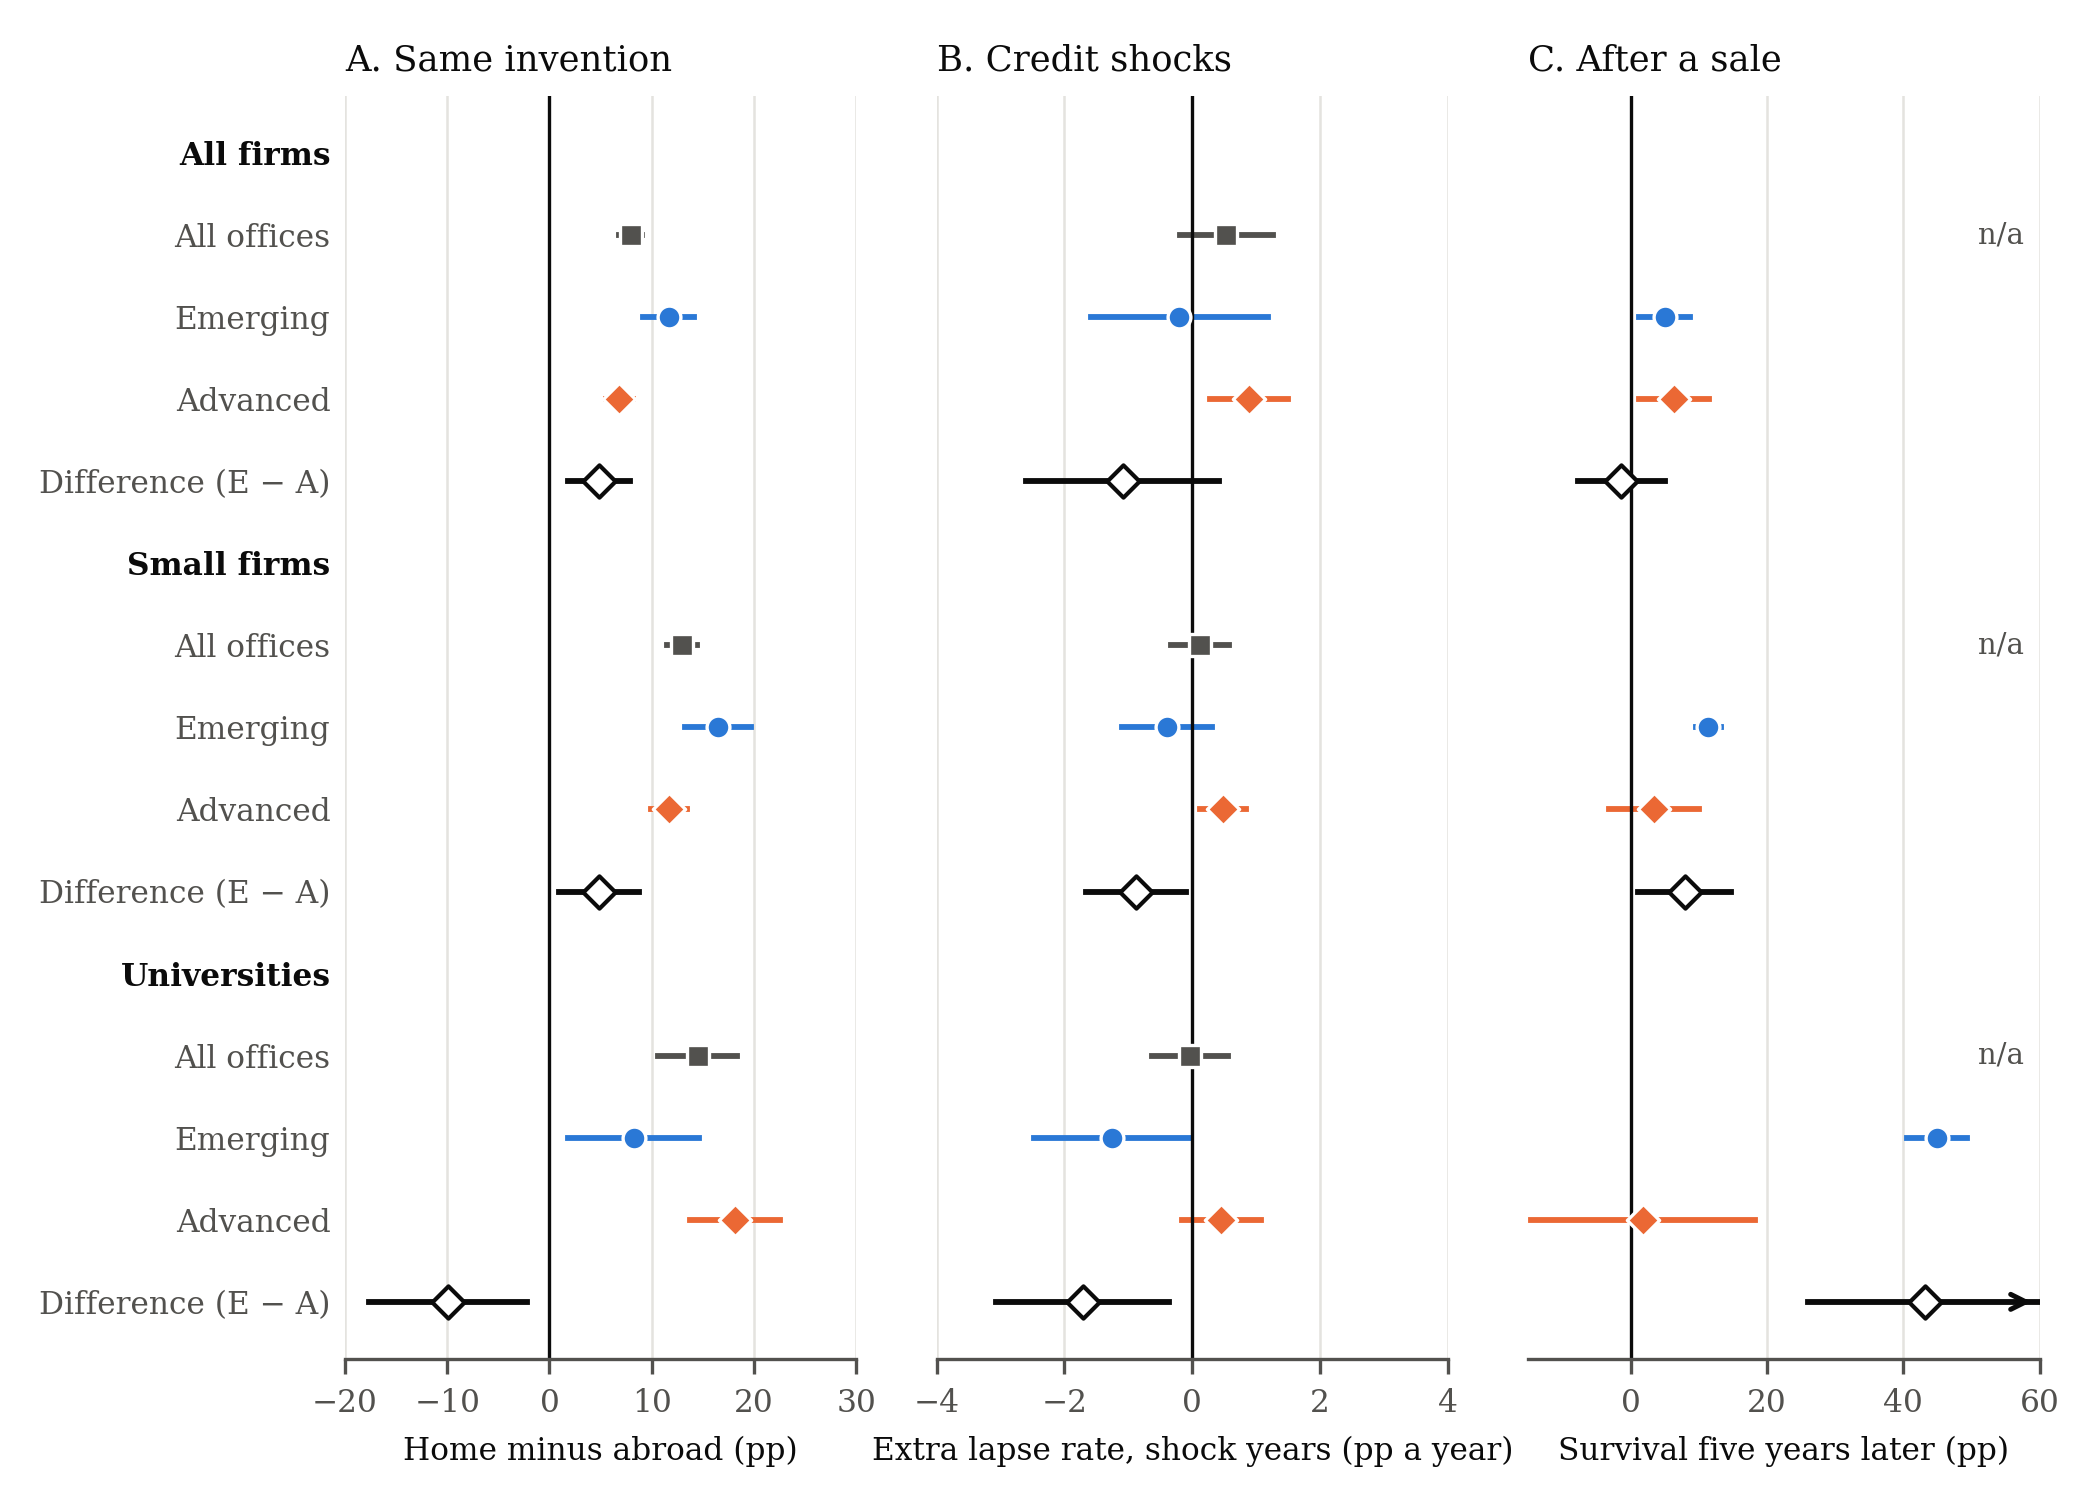
\includegraphics[width=\textwidth]{figures/fig5_constraints.png}
\caption{Three tests for owner constraints}\label{fig:constraints}
\figurenotes{Point estimates with 95\% confidence intervals, in percentage points. Squares: all offices; circles:
emerging economies; diamonds: advanced economies; open diamonds: emerging minus advanced. Small firms: 1--9 inventions
filed worldwide in 2000--2005 by the owner. A: survival eight years after grant of the home patent minus
that of the same invention's patents in other study offices; inventions granted at home and in at least one other
study office, with patent-family and office $\times$ year effects. B: extra yearly lapse rate of domestic owners in
credit-shock years; patents at risk by office, year, age and citation tercile, weighted by patents at risk, with
office $\times$ year, office $\times$ age $\times$ citation-tercile and office $\times$ owner-group $\times$ domestic
effects and standard errors clustered by office $\times$ year. Credit-shock years (systemic banking crises in
\citealp{LaevenValencia2018} and documented credit crunches): 2008--09 in the advanced economies, Taiwan and the
Czech Republic; 2003--04 (credit-card crisis; \citealp{KangMa2009}) and 2008--09 in Korea; 2013 (interbank crunch;
\citealp{BIS2013}) and 2017--18 (deleveraging) in China; 2008--09 and 2014--15 (rouble crisis) in Russia. C: survival
five years later of domestic owners' patents sold to an unrelated buyer 4--8 years after filing minus that of unsold
patents at the same point; emerging: China; advanced: Germany and France, the records that name the new
owner; patents alive and unsold 4--8 years after filing, with landmark-age $\times$ year, field and
owner-group effects, log citations up to the landmark and the grant lag. A and C: standard errors clustered by
owner. Emerging-minus-advanced differences are interactions in one regression.}
\end{figure}

\paragraph{Same invention, home and abroad.} Inventions patented both at home and in another study office hold the
technology fixed. With patent-family fixed effects, owners everywhere keep the home patent longer than the same
invention's foreign patents, by 7.9 points, and small firms by 13.0: the home market is where they use the invention,
and foreign protection is dropped first (panel A). If emerging-market owners found their home patents hard to use,
their home advantage would be smaller. It is larger: 11.7 points against 6.8 in the advanced economies, a difference
of 4.8, and 16.5 against 11.7 for small firms, a difference of 4.9.

\paragraph{Credit shocks.} If finance were binding, credit crunches should raise domestic owners' lapses, and small
firms' most. Following each patent year by year, with country-specific shock years (the notes to Figure~\ref{fig:constraints}), domestic
owners in the advanced economies lapse slightly more in shock years, by 0.9 points a year, and their small firms by 0.5
(panel B). Domestic owners in the emerging economies do not: $-0.2$ for all firms and $-0.4$ for small firms, so the
difference is negative ($-0.9$ for small firms). Each comparison is within an office and year, so fee changes and
recording practices do not drive it.

\paragraph{Sales.} One result points to owner capacity at the margin. I follow patents alive and not yet sold 4--8
years after filing, compare those sold in the next year with those not sold, and record whether they are alive five
years later. Many recorded transfers are renames, restructurings or moves within a group, which say nothing about a
new owner, so I keep only sales to unrelated buyers, identified from the owners' names; only the Chinese, German and
French records carry them (Supplemental Appendix Table~S5). A sale to an unrelated buyer raises the survival of small
Chinese firms' patents by 11.4 points, against 3.5 in Germany and France, a difference of 7.9.
Buyers pick good patents everywhere, so the premium itself does not measure what a sale adds; the informative part is
how much larger it is for small Chinese firm sellers. Because few small German and French firms sell to unrelated
buyers, the difference is imprecise; counted from grant it is 3.7, and with all recorded transfers in the six
offices that record them, 7.0. For mid-sized and large firms there is no difference.

\paragraph{Universities.} Universities behave differently from firms on two of the three tests. Emerging-market
universities keep the home patent 8.2 points longer than the same invention's foreign patents, against 18.2 for
advanced-economy universities, a difference of $-9.9$: unlike firms, they lean less on their home patents. And a sale
to an unrelated firm raises the survival of Chinese university patents by 44.9 points, against almost nothing in
Germany and France. Patents that Chinese universities would have dropped survive in the hands of firms; buyers choose
which patents to buy, so part of the gap is selection, but the same selection operates in the advanced economies,
where there is no premium. Credit shocks do not raise universities' lapses in either group as a whole, as expected for
owners funded by public budgets rather than credit. Together with their lower survival and values at equal quality,
this suggests that for Chinese universities the problem lies partly with the owner: they hold patents that firms find
worth keeping but that they do not use themselves.

\paragraph{Fees.} Fee changes test the cash constraints at renewal time directly, but only small firms receive the
discounts, so the test is small against large firms rather than emerging against advanced. China's fee reduction for
small owners (70\% in the first three fee-years after grant, raised to 85\% and extended to six fee-years in 2016 and
to ten in 2018) barely changes small firms' lapses: a 10\% lower fee lowers their lapse rate, 3.6\% a year, by about
0.2\% of its level, not significantly, measured over all eligible firms because take-up is not observed. Small US
firms respond to changes in the three US maintenance fees about ten times as strongly (2.6\% for a 10\% fee change). Small Chinese firms are not
more fee-sensitive than small US firms.

\section{What the patents are worth}\label{sec:values}

Survival is a coarse measure: it ignores how much fees differ between offices and over a patent's life. Renewal
models turn each patent's fee path and lapse decision into money. Fees come from official schedules for each of the
ten offices by year of life and period, deflated to 2024 prices with each country's consumer price index and
converted at 2024 purchasing-power parities \citep{WDI}.

\paragraph{Two models.} In the deterministic model \citep{SchankermanPakes1986}, a patent earns $r_0 d^t$ in year $t$
after grant: $r_0$ is its return in the year of grant and $d$ the share of returns that carries over to the next
year, so returns decline at rate $1-d$. Initial returns are log-normal, $\ln r_0 \sim N(\alpha_g + \gamma \ln(1+n_i),
\sigma)$, where $n_i$ is the patent's forward citations, $\alpha_g$ the mean log return of owner group $g$
(domestic or foreign $\times$ firm size or university), $\gamma$ the elasticity of returns with respect to citations
and $\sigma$ the standard deviation of log returns. With returns falling and fees rising, the owner renews while
returns over the period a fee covers exceed the fee. In this model the rate of decline $1-d$ is not identified, so I also estimate the
learning model of \citet{Pakes1986}, in which log returns follow a random walk whose shocks shrink as owners learn,
and owners may keep a patent worth less than its fee for the option of later renewals. Where fees rise steeply every year $d$ is identified: 0.850 in Germany, 0.827 in the United Kingdom
and 0.831 in France, close to earlier renewal estimates, which put the decay of returns at 10--20 percent a
year \citep{SchankermanPakes1986,Griliches1990}; elsewhere the rate is not identified. I fix $d = 0.85$ everywhere. Appendix~\ref{app:models} sets out both models; Supplemental Appendix~S4 describes the fee schedules and reports the estimates.

\paragraph{Patent-level values.} Group averages could hide the patents that matter, and they depend on how owners are
grouped. I therefore value each patent from its own renewal history: the learning model is re-estimated with the same
starting distribution of returns for all owners, which depends only on citations, and each patent's value is the
median over simulated return paths, weighting each path by how likely it makes the patent's observed lapse or
survival. Owner type plays no
role in a patent's value. Figure~\ref{fig:valuespooled} compares, for each owner group, the values of domestic and
foreign owners' patents on the same fee path, in the same citation band and in the same field of the same office.\footnote{\label{fn:valuespecs}Each patent's posterior median value at grant from the learning model with a common prior ($d=0.85$; 2024 PPP dollars), regressed on domestic owner $\times$ owner group with fee-path $\times$ citation-band, office $\times$ field and office $\times$ owner-group effects; standard errors
clustered by owner; 1.17 million patents (Russia, and Brazilian patents granted before June 2009, left out). The emerging-minus-advanced difference is an interaction in one regression.}
This is the home premium.

\begin{figure}[!htbp]
\centering
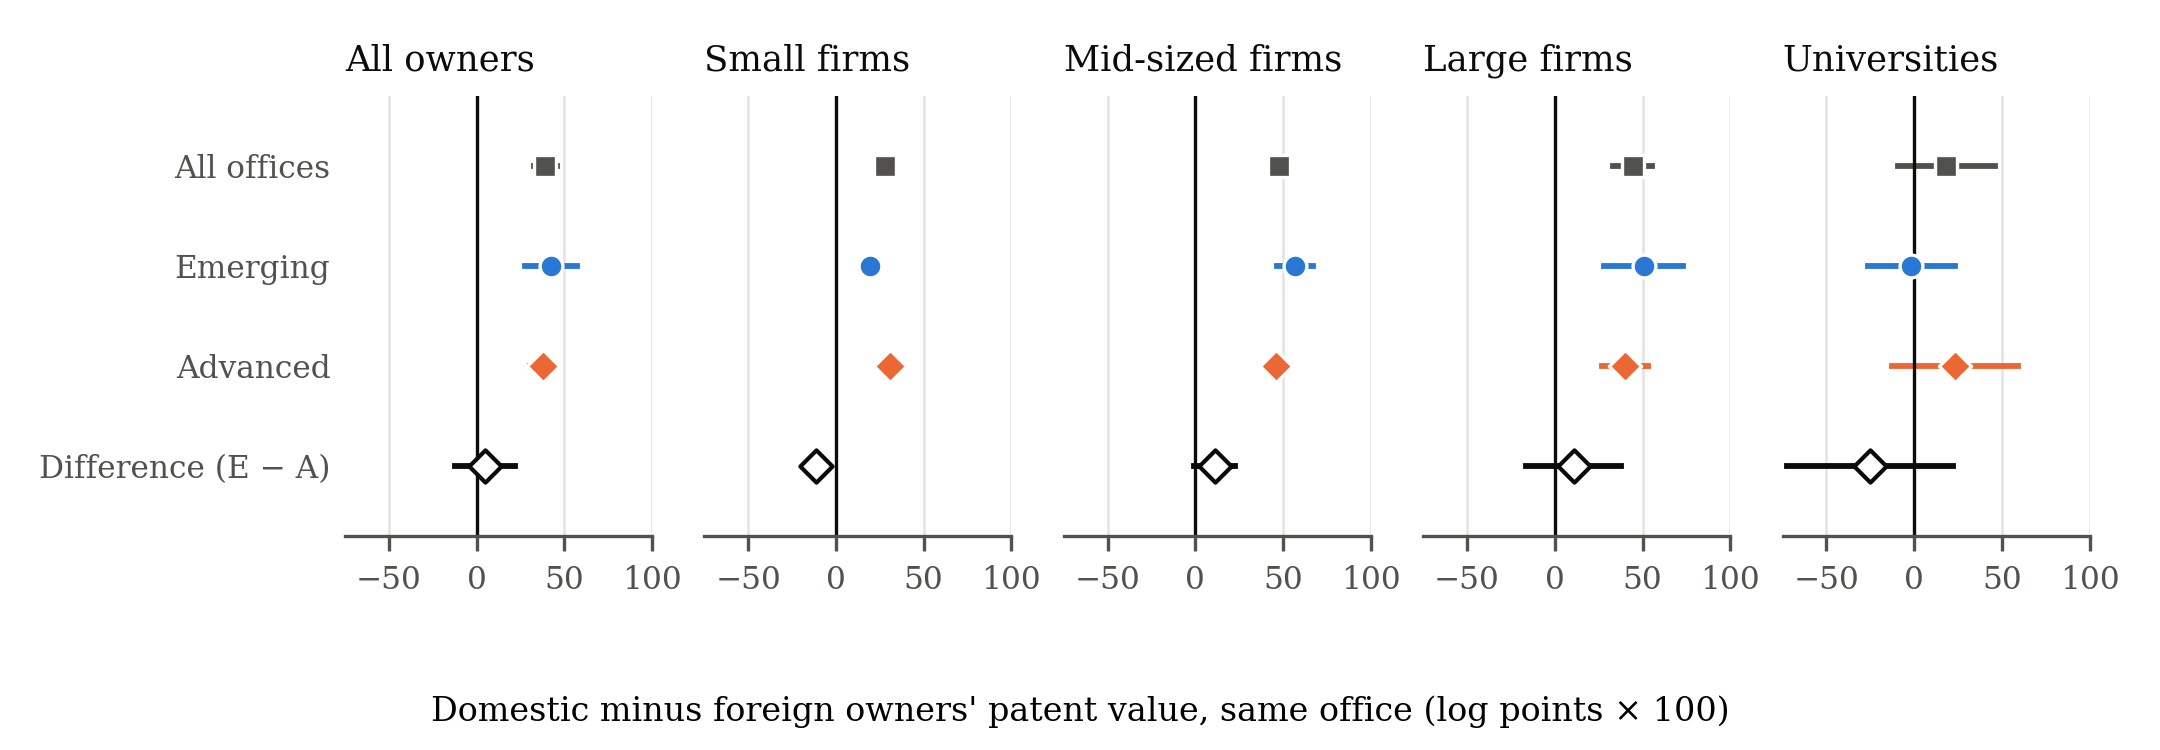
\includegraphics[width=\textwidth]{figures/fig7_values_pooled.png}
\caption{Value of domestic relative to foreign owners' patents, by owner group}\label{fig:valuespooled}
\figurenotes{Point estimates with 95\% confidence intervals, in percent, $100(e^{b}-1)$ for a log-value gap $b$; for the difference, the percentage by which the emerging-market ratio exceeds the advanced one.
Squares: all offices; circles: emerging-market offices (Russia left out, its values not identified); diamonds:
advanced-economy offices; open diamonds: emerging minus advanced. Value: each patent's value at grant estimated from its
own renewal history. Specification in footnote~\ref{fn:valuespecs}.}
\end{figure}

\paragraph{The home premium.} Domestic owners value their patents more than foreign owners in the same office, as
they should: the home market is where they sell. Across all owners the premium is smaller in the emerging-market offices, but not significantly: domestic owners'
patents are worth 31\% more than foreign owners' there\footnote{\label{fn:russia}Russia is left out:
its values are not identified. Domestic owners paid very low fees, about \$50--150 a year in PPP terms, but let many
patents lapse, while foreign owners paid four and a half times the resident fee until 2012 and kept theirs; the model
cannot separate low value from lapses unrelated to the fee.} and 45\% more
in the advanced ones. For mid-sized firms it is larger in the emerging-market offices, 80\% against 58\%; for large
firms it is 37\% against 47\%, not significantly different. Small firms' home premium is 23\% in the
emerging-market offices and 35\% in the advanced ones, 9\% less. As in Section~\ref{sec:survival}, the benchmark matters. Small
Japanese firms value their home patents far above foreign owners do in Japan (226\% more), and Japan contributes a
large share of the advanced-economy patents. Office by office, the premium of small firms is 29\% in China and
65\% in Korea, against 28\% in the United States, 31\% in Germany and 8\% in the United Kingdom; it is 7\% in Brazil,
imprecisely, and close to zero in the Czech Republic and France (Supplemental Appendix Table~S8). Universities are the exception among
emerging-market owners: Chinese universities' patents are worth 59\% less than foreign universities' patents in China
($1-e^{-0.88}$). The deterministic model and other decay rates give the same pattern (Supplemental Appendix~S4).

\paragraph{Fee discounts do not change the comparison.} China and Korea cut renewal fees for domestic small firms and
universities (as does Brazil), and the models above assume standard fees. Lower fees mean the same renewal behaviour implies lower
values, so I re-estimate both models for China and Korea assuming that every eligible owner took the discount: in China, 30\% of the fee
in the first three fee-years after grant until 2016, then 15\% for six fee-years and, from 2018, for ten; in Korea, 70\% of the fee
in years 4--6 from 2014 and half from 2018. The ratio of small domestic to
small foreign firms' median value at equal citations barely moves: from 2.04 to 1.99 in China and from 2.72 to 2.63 in
Korea in the deterministic model, and from 1.95 to 1.98 and from 2.31 to 2.08 in the learning model. 

\paragraph{Levels are rough; comparisons are not.} A typical small domestic firm's patent is worth roughly
\$5{,}000--62{,}000 at grant in the deterministic model and more, in some offices several times more, in the learning model, in which early
lapses reflect learning rather than low initial value. Values in different offices also cover protection in
different markets. The comparisons between owners, on which the argument rests, are stable across models, decay rates
and fee assumptions, except in Russia. Because a patent's value on a given fee path rises with how long it is kept,
the patent-level values restate the survival results in money.

\section{What is at stake? Three policy levers}\label{sec:stake}

The introduction set out two families of policy: if the invention is the problem, invest in research capability; if
the inventor is, relieve owners' constraints through credit, fee relief or markets for technology. The renewal model
can price the levers that the evidence points to on a common scale. I simulate each patent on its own fee path to
expiry with the deterministic model of Section~\ref{sec:values}, change one thing at a time, and report the change
in the returns owners earn from their patents per filing-year cohort, in 2024 PPP dollars and as a share of national
R\&D spending, for China, Korea and Brazil (Table~\ref{tab:levers}).\footnote{\label{fn:levers}China, Korea and Brazil are the three emerging-market
offices with fee discounts for small owners, which the first lever needs. Korea records no sales of granted patents
and Brazil's records, which name the new owner, show too few sales of granted patents by domestic owners to unrelated buyers (8 at the
ages studied), so markets for technology are priced for China only. The Czech
Republic records no ownership transfers and has no fee discount for small owners, and the Russian values are not
identified (Section~\ref{sec:values}). Patents a year: in China 4{,}100 of
small firms, 1{,}800 of mid-sized firms, 5{,}200 of large firms and 6{,}600 of universities; in Korea 4{,}700, 3{,}800,
26{,}900 and 3{,}300; in Brazil 45, 20, 18 and 43. Firm size: inventions filed worldwide in 2000--2005 by the owner. National R\&D: gross domestic expenditure on
R\&D, 2000--2005 average \citep{WDI}. Decay factor $d = 0.85$; fees after 2024 at 2024 prices. Fee relief: every eligible
owner (firms with fewer than 100 inventions, universities) pays the discounted fees; in Brazil 40\% of the
standard annuity (50\% from August 2025), simulated for patents granted from June 2009, whose fees are known. Markets for technology:
returns multiplied, from one year after grant, by a factor calibrated so that the model's survival five years after a
sale, 1--5 years after grant, rises by the extra post-sale survival of sales to unrelated buyers in China relative to
Germany and France, counted from grant: 3.8 points for small firms and 4.8 for mid-sized firms,
giving factors of 1.22 and 1.40; none for large firms. For universities the factor, 3.5, matches Chinese
universities' own premium of 46 points less the 7 points in Germany and France. University patenting: mean log returns of Chinese
universities raised to those of foreign universities in China (upper bound) or to the foreign level plus the average
domestic--foreign university gap in the United States, Germany, the United Kingdom and France (lower bound).} Fees saved are transfers from the state to owners,
so they are not counted in the table.

\paragraph{Fee relief.} Suppose every eligible owner (firms with fewer than 100 inventions and universities) took up
the Chinese, Korean and Brazilian fee discounts. Owners of a Chinese cohort would pay \$8.0 million less in fees,
owners of a Korean one \$1.8 million less and owners of a Brazilian one \$0.2 million less, but they would keep their
patents only marginally longer, and the returns they earn would rise by about half a million dollars in China, 1.3
million in Korea and 0.1 million in Brazil. Fees are small relative to what patents are worth, so cutting them
changes few renewal decisions. Brazil is the partial exception: its patents are worth little relative to its fees,
and the discount would raise the value of eligible owners' patents by 37--50\%, but they hold only about 110 patents
a cohort.

\paragraph{Markets for technology.} Suppose that, from one year after grant, domestic owners' patents earned what they
would earn in the hands of a buyer. For each group I calibrate the buyer's advantage to the extra survival of patents sold to
unrelated buyers in Section~\ref{sec:constraints}, relative to sellers of the same size in Germany and France,
counted from grant to match the model. In China this requires returns about 20\% higher for small firms and 40\% for
mid-sized firms, and the returns from a cohort of small firms' patents would rise by about \$130 million, or \$280
million with mid-sized firms. Both targets are imprecise, so these are orders of magnitude; large firms show no
premium. Korea records no sales of granted patents, so the lever is not priced there. For Chinese universities, whose
sold patents survive 45 points longer, the calibrated advantage is a 3.5-fold increase in returns and the gain
\$460 million. Each figure is an upper bound, since it reallocates every patent of the group.

\paragraph{University patenting.} Suppose instead that Chinese universities' patents earned what foreign
universities' patents earn in China at equal citations. Each cohort would be worth about \$320 million more; with
the typical university home premium of the advanced-economy offices as the benchmark, about \$180 million. This and
the university row under markets for technology are two routes to the same lost value, improving what universities
patent or moving their patents to owners who use them, and should not be added.

\begin{table}[t]
\centering
\begin{threeparttable}
\caption{Returns at stake per filing-year cohort, by lever and owner group (millions of 2024 PPP dollars)}\label{tab:levers}
\small
% Generated by em-patent-value code/38_paper_exhibits.py (policy_levers.csv, step 26); do not edit by hand
\begin{tabular}{lccccc}
\toprule
 & \multicolumn{3}{c}{Fee relief} & Markets for technology & University patenting \\
\cmidrule(lr){2-4}\cmidrule(lr){5-5}\cmidrule(lr){6-6}
 & China & Korea & Brazil & China & China \\
\midrule
Small firms (1--9)          & 0.07 & 0.49 & 0.05 & 133 &  \\
Mid-sized firms (10--99)    & 0.02 & 0.42 & 0.03 & 146 &  \\
Large firms (100+)          & n.e. & n.e. & n.e. & 0.00 &  \\
Universities                & 0.43 & 0.34 & 0.04 & 462 & 178--319 \\
\addlinespace
All owners                  & 0.52 & 1.3 & 0.11 & 742 & 178--319 \\
\quad \% of national R\&D & 0.00 & 0.00 & 0.00 & 0.79 & 0.19--0.34 \\
\bottomrule
\end{tabular}
\begin{tablenotes}\footnotesize
\item \emph{Notes:} Change in the returns domestic owners earn from their patents, excluding fees, for one filing-year cohort; deterministic renewal model, each patent simulated on its own fee path. Markets for technology: upper bounds, calibrated to the extra post-sale survival of arm's-length sales; the firm targets are imprecise (\SuppTab{S5}{tab:sales}). The two university entries are alternative routes to the same value and are not additive. n.e.: not eligible. Details in footnote~\ref{fn:levers}.
\end{tablenotes}
\end{threeparttable}
\end{table}


\paragraph{Reading the numbers.} Two cautions apply. The figures are private returns to owners, not welfare: they
leave out knowledge spillovers and the gain to users when a patent enters the public domain. The levels are rough: the
decay rate is fixed rather than estimated in China, the sale targets are imprecise, and in the learning model, where
owners keep low-value patents for the option of later renewals, the same survival gains require far larger changes in
returns and give levels several times higher that are not identified (Supplemental Appendix Table~S9). The ordering survives both: relieving owners of fees is worth
about a million dollars a cohort or less, while helping patents reach owners who can use them and improving what Chinese
universities patent are worth hundreds of millions, two to three orders of magnitude more.

\section{Conclusion}\label{sec:conclusion}

The emerging-market shortfall in patent survival reflects what gets patented. At equal observable quality and grant
lag, firms in China, Korea and Taiwan keep their patents at least as long as comparable firms in the United States,
Japan, Germany, the United Kingdom and France, and value them about as much relative to foreign owners. On average,
credit shocks and fee cuts barely move their renewal decisions, and they keep the home patents of their inventions
longer than the foreign ones. For firms, the binding constraint is the invention, not the inventor.

Two qualifications matter for policy, and the counterfactuals put a rough price on both. Owner capacity counts at the
margin: patents that small Chinese firms sell to unrelated buyers survive much longer, and moving such patents to
owners able to use them is worth up to \$130--280 million per cohort in China. Policies that deepen markets for
technology, such as registries, licensing intermediaries and secure transfer of title, may therefore add value, while
fee relief, worth almost nothing on the same scale, is unlikely to change which patents are kept. And Chinese
universities are a clear weak spot: their patents are dropped sooner and are worth less than half as much as
comparable foreign ones, consistent with patenting driven by evaluation and subsidy targets rather than use. Yet once
sold to firms, the same patents survive far longer, so part of the loss lies in who holds them: technology-transfer
offices and licensing to firms may recover much of the value, worth \$180--460 million per cohort. Russia, where
domestic patents fall well behind, deserves a closer look.

Three limitations stand out. Only five emerging economies record lapses well enough to study, and two of them, Korea
and Taiwan, are now high-income. The firm results rest on citations to the whole patent family; with citations from
the same office only, emerging-market firms are somewhat behind. And renewal values measure private value to the
owner, not the social value of the knowledge a patent spreads.


% In-paper appendix: starts on a new page after the text and before the references (counts toward the word limit)
\clearpage
\appendix
\section{Renewal models}\label{app:models}

Fee schedules, the fee discounts and the estimates are in Supplemental Appendix~S4.

\paragraph{Deterministic model.} A patent earns $r_0 d^t$ in year $t$ after grant. At decision $j$, at time $t_j$,
the owner pays $c_j$ to keep the patent for $L_j$ years and renews if
$r_0 d^{t_j} \sum_{s<L_j} (\beta d)^s \ge c_j$, i.e.\ if $r_0 \ge \tau_j$. With returns falling and fees rising
this rule is optimal, and a patent survives decision $j$ if $r_0 \ge \max_{l\le j}\tau_l$. In addition, at each
decision the owner drops the patent with probability $h = 1\%$ for reasons unrelated to value. With
$\ln r_0 \sim N(\alpha_g + \gamma \ln(1+c), \sigma)$, the likelihood of each patent's lapse or censoring decision
follows directly. The discount factor is $\beta = 0.9$. Estimation is by maximum likelihood, office by office, on up
to 60{,}000 patents per owner group.

\paragraph{Learning model.} Log returns $x_t$ start at $x_0 \sim N(\mu_i, \sigma_0)$ and evolve as
$x_{t+\Delta} = x_t + \Delta \ln d + e$, with $e \sim N\big(0,\, s^2(\varphi^{2t}-\varphi^{2(t+\Delta)})/(-2\ln\varphi)\big)$:
a random walk with drift whose shocks shrink at rate $\varphi$ as the owner learns. The value of a patent at decision
$j$ solves
\[
V_j(x) = \max\Big\{0,\; e^x \sum_{u<L_j} (\beta d)^u - c_j + \beta^{t_{j+1}-t_j} (1-h)\, E\,V_{j+1}(x')\Big\},
\]
so a patent may be kept below its current fee for the option of later renewals. Thresholds come from backward
induction on a grid for each fee path, run to expiry. Expectations use Gauss--Hermite quadrature. Survival is
simulated with common random numbers and a smoothed renewal indicator, and the likelihood is built from lapse and
censoring counts in cells of fee path $\times$ owner group $\times$ citation band. Supplemental Appendix
Table~S6 reports the estimates.

\paragraph{Patent-level values.} For the values of Section~\ref{sec:values}, the learning model is re-estimated with a single prior for all owners
($\mu_i$ depends on the citation band only). For each cell, 1{,}000 return paths are simulated; a patent that lapsed at
decision $k$ weights each path by the probability of surviving to $k-1$ and lapsing at $k$, and a patent still alive
at the end of the data by the probability of surviving all observed decisions, plus the value of optimal renewals
after the data end. A patent's value is the weighted median over paths.


\bibliographystyle{plainnat}
\ifdefined\aeriwordcount
\nobibliography{references}
\else
\clearpage
\bibliography{references}
\fi

\end{document}
